\documentclass[12pt, a4paper]{article}

% ── Packages ──────────────────────────────────────────────────
\usepackage[utf8]{inputenc}
\usepackage[T1]{fontenc}
\usepackage{lmodern}
\usepackage[margin=1in]{geometry}
\usepackage{amsmath, amssymb, amsthm}
\usepackage{graphicx}
\usepackage{hyperref}
\usepackage{xcolor}
\usepackage{enumitem}
\usepackage{booktabs}
\usepackage{caption}
\usepackage{subcaption}
\usepackage{fancyhdr}
\usepackage{listings}
\usepackage{textcomp}
\usepackage{tikz}
\usetikzlibrary{arrows.meta, positioning, calc, shadows.blur, decorations.markings, backgrounds, fit, shapes.symbols}

% ── Page style ────────────────────────────────────────────────
\setlength{\headheight}{14.5pt}
\addtolength{\topmargin}{-2.5pt}
\pagestyle{fancy}
\fancyhf{}
\rhead{\thepage}
\lhead{\leftmark}

% ── Hyperlink colors ─────────────────────────────────────────
\hypersetup{
    colorlinks=true,
    linkcolor=blue!70!black,
    citecolor=green!50!black,
    urlcolor=blue!60!black,
}

% ── Theorem environments ─────────────────────────────────────
\newtheorem{theorem}{Theorem}[section]
\newtheorem{lemma}[theorem]{Lemma}
\newtheorem{definition}[theorem]{Definition}

% ── Code listing style ───────────────────────────────────────
\lstset{
    language=Python,
    basicstyle=\small\ttfamily,
    keywordstyle=\color{blue!70!black},
    commentstyle=\color{green!50!black},
    stringstyle=\color{red!60!black},
    breaklines=true,
    frame=single,
    numbers=left,
    numberstyle=\tiny\color{gray},
    xleftmargin=2em,
    framexleftmargin=1.5em,
    captionpos=b,
}

% ── Title ─────────────────────────────────────────────────────
\title{\textbf{ManiBench}\\[0.3em]
       \large A Benchmark for Testing Visual-Logic Drift and Syntactic\\
       Hallucinations in Manim Code Generation}
\author{Oli, Nabin}
\date{\today}

% ══════════════════════════════════════════════════════════════
\begin{document}
\maketitle

\begin{abstract}
Traditional code-generation benchmarks like HumanEval and MBPP excel at testing logic and syntax, but they fall short when code must translate into dynamic, pedagogical visuals.
We introduce \textsc{ManiBench}, a specialized benchmark designed to evaluate LLM performance in generating Manim~CE (Community Edition) code---a domain where temporal fidelity and version-aware API correctness are paramount.
\textsc{ManiBench} addresses two critical failure modes prevalent in LLM outputs:
\emph{Syntactic Hallucinations} (generating code that is grammatically valid Python but references non-existent Manim functions, outdated or deprecated APIs, undefined classes, or calls that break under specific library versions) and
\emph{Visual-Logic Drift} (occurrences where generated visuals diverge from intended mathematical logic, such as missing events, incorrect causal relationships, timing errors, or the model struggling to animate a concept).
The benchmark aims to collect 150--200 problems, launching with a pilot of 12~high-quality challenges across five difficulty levels.
These span domains including calculus, linear algebra, probability, topology, and AI\@.
Task types are uniquely structured into categories such as drift-sensitive transformations, debugging, version-conflict traps, and multi-scene narratives.
Each problem is backed by reference code analysis of the original 3Blue1Brown ManimGL source (${\sim}53{,}000$~lines total, 143~scene classes, 145~documented GL$\to$CE incompatibilities).
To move beyond simple test-case-based checks, \textsc{ManiBench} employs a four-tier scoring framework:
(1)~\emph{Executability} (Pass@1): the fraction of outputs running without exceptions or deprecated imports;
(2)~\emph{Version-Conflict Error Rate}: the frequency of runs triggering mixed-API or legacy errors;
(3)~\emph{Alignment Score}: the weighted fraction of required visual events that are both present and temporally accurate; and
(4)~\emph{Coverage Score}: a four-dimensional measure of pedagogical element density spanning mathematical annotations, visual mapping, numeric evidence, and structural clarity.
An accompanying open-source evaluation framework automates metric computation across models from multiple providers and five prompting strategies.
By formalizing the requirements for temporal and syntactic precision, \textsc{ManiBench} provides a foundational testbed for the next generation of automated educational content and visual-logic synthesis.
\end{abstract}

\noindent\textbf{Keywords:} Syntactic Hallucinations, Visual-Logic Drift, Manim~CE, Code Generation, Benchmarking

\tableofcontents
\newpage


%% ═══════════════════════════════════════════════════════════════
\section{Introduction}
\label{sec:introduction}

The rise of large language models (LLMs) has accelerated research in code generation. Benchmarks such as HumanEval, MBPP, and APPS are commonly used to evaluate LLM coding ability~\cite{}. These benchmarks emphasize logical correctness, syntactic validity, and output matching—i.e., whether generated code solves the task, executes without errors, and yields the expected results. While well suited for algorithmic problems, these criteria are insufficient for domains in which code produces continuous, time-dependent visual outputs.

Manim, a Python animation engine developed by Grant Sanderson (3Blue1Brown), constructs mathematical animations by composing scene objects, applying geometric and visual transformations, and controlling timing. A Manim script may be syntactically valid yet fail to convey the intended concept; we identify three common failure modes:
\begin{itemize}[nosep]
    \item \textbf{Incorrect visual semantics:} animations move in unintended directions or transform the wrong objects.
    \item \textbf{Timing misalignments:} events occur out of order or at inappropriate times, breaking causal or pedagogical flow.
    \item \textbf{Pedagogical failure:} animations obscure rather than clarify the concept (missing annotations, poor sequencing, or absent explanatory cues).
\end{itemize}

Manim exists in major two variants. Manim~CE (Community Edition) is an actively maintained, open-source implementation with a modern API, whereas Manim~GL (the original 3B1B fork) contains deprecated constructs and hand-optimized code paths. LLMs frequently conflate APIs across these variants or reference renamed/moved functions, producing code that fails under particular library versions~\cite{}.


\subsection{Related Work}
\label{sec:related}

\subsubsection{Code Generation Benchmarks}
\label{sec:codegenBench}

Evaluation of large language models (LLMs) for program synthesis has progressed from function-level correctness to repository-scale reasoning. Early benchmarks such as \textbf{\textit{HumanEval}}~\cite{} formalized unit-test-based validation through the Pass@k metric, establishing executability as the primary indicator of correctness. \textbf{\textit{MBPP}}~\cite{} extended this setting to natural-language-to-code tasks across entry-level Python problems. More recent benchmarks such as \textbf{\textit{DS-1000}}~\cite{} incorporated third-party library usage, while \textbf{\textit{SWE-Bench}} introduced repository-scale issue resolution requiring multi-file contextual reasoning.


\begin{table}[ht]
    \centering
    \caption{Comparison of related benchmarks and limitations addressed by \textsc{ManiBench}.}
    \label{tab:related-benchmarks}
    \small
    \begin{tabular}{@{}lp{3.6cm}p{2.6cm}p{6.2cm}@{}}
        \toprule
        \textbf{Benchmark} & \textbf{Focus / Area} & \textbf{Primary Metric} & \textbf{Limitation Addressed by ManiBench} \\
        \midrule
        HumanEval / MBPP~\cite{} & Python program synthesis, algorithmic tasks & Pass@k (logic correctness) & Temporal fidelity: these benchmarks lack rendering; code can pass logic tests yet fail to animate concepts over time. \\
        \addlinespace
        SWE-Bench~\cite{} & Software engineering / repo-level edits & Unit test / patch pass rate & Visual-logic drift: fixes that satisfy tests may still produce visuals that diverge from mathematical intent. \\
        \addlinespace
        DSCodeBench~\cite{} & Data-science APIs and pipelines & API coverage / correctness & Version hallucination: evolving third-party APIs cause models to generate deprecated or mismatched calls; ManiBench tracks 145+ GL$\to$CE incompatibilities. \\
        \addlinespace
        Code2Video (2025)~\cite{} & Educational video/storyboarding & Teach-quiz / aesthetic scoring & Syntactic hallucination: Code2Video emphasizes storyboarding and high-level layout, but does not drill into broken or versioned API calls in animation frameworks. \\
        \addlinespace
        SVGenius (2025)~\cite{} & SVG editing / static visual generation & Visual-structural scoring & Multi-scene narratives: SVG-focused benchmarks do not evaluate complex temporal causal relationships across multiple animation scenes as ManiBench does. \\
        \bottomrule
    \end{tabular}
\end{table}


Despite increasing scale and realism, these benchmarks remain fundamentally test-driven~\cite{}. Solutions are considered correct if they pass predefined unit tests or patch validation suites~\cite{}. This evaluation paradigm does not account for renderable behavior, temporal sequencing, or alignment between code structure and intended visual semantics. In animation scripting environments, code may execute without error yet still fail to convey the intended conceptual narrative. This limitation motivates evaluation beyond executability.

\subsubsection{Visual-Logic Drift in Executable Code}

In renderable programming domains, correctness extends beyond runtime validity to semantic alignment between generated output and instructional intent. We define \textbf{\textit{visual-logic drift}} as the divergence between the intended mathematical narrative and the rendered animation, even when code executes successfully. Unlike traditional logical errors, drift may arise from subtle structural mismatches: incorrect object transformations, missing intermediate states, improper sequencing of animation calls, or violations of causal dependencies across scenes.

Existing visual-code benchmarks primarily focus on static artifact generation (e.g., vector graphics or diagram editing), where evaluation centers on structural similarity. Animation scripting introduces temporal constraints and multi-step causal structure, requiring preservation of event ordering and pedagogical coherence. Current benchmarks do not quantify this form of semantic drift in executable animation environments.

\subsubsection{Syntactic Hallucinations and Version Conflicts}

Hallucination in code generation has been widely characterized as the production of syntactically valid but semantically incorrect outputs, including fabricated APIs, deprecated function usage, and identifier conflicts. Prior work demonstrates that hallucination rates increase in low-frequency or evolving libraries, and that such errors often evade static analysis because they remain grammatically valid Python.

In rapidly evolving libraries, version misalignment introduces an additional layer of failure. Models may generate code consistent with legacy documentation while the prompt implicitly assumes a newer API specification. These errors are particularly difficult to detect in animation frameworks, where partial execution may mask deeper incompatibilities. Existing hallucination research quantifies runtime failures but does not evaluate how version conflicts propagate into higher-level structural inconsistencies.

\subsubsection{Positioning \textbf{\textit{ManiBench}}}

\textbf{\textit{ManiBench}} is situated at the intersection of code-generation benchmarking, hallucination analysis, and visual-temporal reasoning. While prior benchmarks evaluate executability and repository-scale edits, and hallucination studies analyze API-level inconsistencies, none jointly assess version-aware API correctness and temporal visual alignment in mathematical animation scripting. \textbf{\textit{ManiBench}} addresses this gap through drift-sensitive task design and a multi-tier evaluation framework that extends beyond unit-test validation to measure semantic fidelity in renderable educational code.


%%%%%%%%%%%%%%%%%%%%%%%%%%%%%%%%%%%%%%%%%%%%%%%%%%%%%%%%%%%%%%%%%%%%%%%%%%%%%%%%%%%%%%%%%%%%%%%%%%%%%%%%%%%%%%%%%%%%%%%%%%%%%%%%%%%%%%%%%%%%%%%%%%%%%%%%%%%%%%%%%%%%%%%%%%%

\subsection{Contributions}
\label{sec:contributions}

\textsc{ManiBench} makes four key contributions:

\begin{enumerate}[nosep]
    \item \textbf{Formalized Visual-Logic Metrics.}
    We define an \emph{Alignment Score} and a four-dimensional \emph{Coverage Score} to capture whether generated animations match pedagogical intent, beyond mere syntactic validity.

    \item \textbf{Version-Aware Evaluation.}
    We explicitly test version-conflict errors and deprecated API usage, with 145~documented GL$\to$CE incompatibilities across eight categories, measuring whether code adheres to a specific Manim version's API contract.

    \item \textbf{Curated Pilot Dataset with Reference Code Analysis.}
    We provide 12~hand-crafted benchmark problems drawn from 3Blue1Brown's published videos, backed by comprehensive analysis of ${\sim}53{,}000$~lines of original source code including 143~scene classes, 120~visual techniques, and detailed visual-event specifications.

    \item \textbf{Automated Evaluation Framework.}
    We release an open-source evaluation pipeline supporting six LLMs across five prompting strategies, with automated metric computation for executability, version conflicts, alignment, and coverage.
\end{enumerate}


%% ═══════════════════════════════════════════════════════════════
% \section{Problem Definition}
% \label{sec:problem}

% \subsection{The Two Failure Modes}
% \label{sec:failure-modes}

% \subsubsection{Syntactic Hallucinations}

% An LLM generates code that:
% \begin{itemize}[nosep]
%     \item references non-existent classes (e.g., \texttt{VMobject} with incorrect spelling);
%     \item uses deprecated functions (e.g., \texttt{mobject.scale()} instead of \texttt{mobject.scale\_to\_fit\_width()});
%     \item calls methods with incorrect signatures;
%     \item mixes Manim~GL syntax with Manim~CE (e.g., using OpenGL-specific rendering calls in~CE).
% \end{itemize}

% \noindent\textbf{Example:}
% \begin{lstlisting}[caption={Syntactic hallucination examples.}]
% # HALLUCINATED: class does not exist
% circle = MCircle(color=BLUE)  # Should be Circle

% # HALLUCINATED: deprecated method
% circle.apply_matrix([[1, 0], [0, 1]])
% # CE removed in favor of apply_complex_function
% \end{lstlisting}

% \subsubsection{Visual-Logic Drift}

% An LLM generates code that:
% \begin{itemize}[nosep]
%     \item omits required visual events (e.g., gradient descent step without showing dot movement);
%     \item implements events in the wrong order (e.g., loss curve updates before parameter updates);
%     \item uses incorrect timing (animations too fast, pauses missing);
%     \item fails to show causal relationships (e.g., showing a result without showing the derivation).
% \end{itemize}

% \noindent\textbf{Example:}
% \begin{lstlisting}[caption={Visual-logic drift example.}]
% # DRIFTED: Gradient descent without showing step updates
% def construct(self):
%     # Shows loss curve but dot doesn't move downhill
%     loss_curve.animate.points = new_points
%     # Missing: dot.animate.move_to(new_point)
% \end{lstlisting}


%%%%%%%%%%%%%%%%%%%%%%%%%%%%%%%%%%%%%%%%%%%%%%%%%%%%%%%%%%%%%%%%%%%%%%%%%%%%%%%%%%%%%%%%%%%%%%%%%%%%%%%%%%%%%%%%%%%%%%%%%%%%%

\section{Problem Definition}
\label{sec:problem}

% \subsection{Primary Failure Modes in Manim Generation}
% \label{sec:failure-modes}

We identify two distinct failure modes that traditional code-generation benchmarks fail to capture when evaluating dynamic visual outputs: \textit{Syntactic Hallucinations} and \textit{Visual-Logic Drift}.

\subsection{Syntactic Hallucinations}
\label{sec:syntactic-hallucinations}

Syntactic hallucinations occur when an LLM produces code that is grammatically valid Python but semantically invalid within the target Manim~CE environment. This failure mode typically manifests when the model:
\begin{itemize}[nosep]
    \item \textbf{Invokes non-existent classes}: e.g., inventing \texttt{MCircle} instead of utilizing the standard \texttt{Circle} class;
    \item \textbf{Employs deprecated methods}: e.g., relying on outdated API calls like \texttt{mobject.scale()} rather than the modern \texttt{mobject.scale\_to\_fit\_width()};
    \item \textbf{Generates incorrect method signatures}: passing unsupported arguments to valid functions;
    \item \textbf{Conflates API versions}: mixing Manim~GL syntax with Manim~CE, such as utilizing OpenGL-specific rendering commands that crash the CE pipeline.
\end{itemize}

\noindent\textbf{Example:}
\begin{lstlisting}[language=Python, caption={Examples of syntactic hallucinations involving hallucinated classes and deprecated methods.}]
# HALLUCINATION: The 'MCircle' class does not exist in Manim CE.
circle = MCircle(color=BLUE)  # Expected: Circle(color=BLUE)

# HALLUCINATION: Deprecated method usage.
# Manim CE favors apply_complex_function over apply_matrix for certain transforms.
circle.apply_matrix([[1, 0], [0, 1]])
\end{lstlisting}

\subsection{Visual-Logic Drift}
\label{sec:visual-logic-drift}

Visual-logic drift emerges when the generated code executes without runtime exceptions but fails to accurately represent the intended mathematical or pedagogical concepts. This semantic decoupling occurs when the model:
\begin{itemize}[nosep]
    \item \textbf{Omits critical visual events}: e.g., illustrating a gradient descent step but failing to animate the corresponding coordinate updates;
    \item \textbf{Inverts sequential logic}: e.g., rendering loss curve updates prior to the parameter adjustments that cause them;
    \item \textbf{Misaligns temporal dynamics}: employing inappropriate animation runtimes or omitting essential pedagogical pauses;
    \item \textbf{Obscures causal relationships}: displaying a final mathematical result without visually articulating the intermediate derivation steps.
\end{itemize}

\noindent\textbf{Example:}
\begin{lstlisting}[language=Python, caption={An example of visual-logic drift where the underlying math is disconnected from the visual output.}]
# DRIFT: Executing a gradient descent step without showing the dot's movement.
def construct(self):
    # The loss curve updates, but the pedagogical link is broken
    # because the representative dot remains static.
    loss_curve.animate.points = new_points
    
    # Missing critical visual event:
    # self.play(dot.animate.move_to(new_point))
\end{lstlisting}

% \subsection{Evaluation Challenges}
% \label{sec:challenges}

% \begin{description}[nosep]
%     \item[Subjectivity of ``correct.'']
%     What counts as a correct gradient descent animation?
%     Must the dot move along the loss surface?
%     Must the curve update dynamically?
%     Must the learning rate shrink?

%     \item[Version fragmentation.]
%     A script that passes in Manim~CE may fail in Manim~GL\@.
%     We must specify which version(s) the code targets.

%     \item[Temporal semantics.]
%     Unlike static code output (e.g., classification accuracy), animations have temporal semantics.
%     An event can be present but timed incorrectly, creating pedagogical failure.
% \end{description}

\subsection{Evaluation Challenges}
\label{sec:challenges}
Evaluating animation code is challenging because correctness is subjective—animations can be syntactically valid yet pedagogically misleading. Version fragmentation means code may run in Manim~CE but fail in Manim~GL. Additionally, temporal semantics matter: events may exist but occur at the wrong time, breaking the intended instructional narrative.


%% ═══════════════════════════════════════════════════════════════



\section{Benchmark Design}
\label{sec:design}
To evaluate generated Manim scripts, we first measure Executability, capturing whether code runs without errors or deprecated usage. This metric establishes a baseline: only scripts that execute successfully can be meaningfully assessed for visual fidelity, timing, and pedagogical alignment.

\subsection{Metric Definitions}
\label{sec:metrics}

\subsubsection{Metric~1: Executability (Pass@1)}

\begin{definition}[Executability]
The fraction of generated outputs that run without raising exceptions or using deprecated imports:
\begin{equation}
    \text{Executability} = \frac{\text{number of successful executions}}{\text{number of total attempts}}.
\end{equation}
\end{definition}

\noindent\textbf{Success criteria:}
\begin{itemize}[nosep]
    \item Script completes without runtime exception.
    \item No deprecated imports detected (scanned via regex or AST analysis).
    \item No warnings from Manim's deprecation system.
\end{itemize}

\noindent\textbf{Failure cases:}
\begin{itemize}[nosep]
    \item Import error (e.g., \texttt{from manim import NonExistent}).
    \item Runtime \texttt{AttributeError} (e.g., \texttt{mobject.invalid\_method()}).
    \item Type error (e.g., passing the wrong type to a function).
    \item Unhandled exception during scene rendering.
\end{itemize}

\subsubsection{Metric~2: Version-Conflict Error Rate}

\begin{definition}[Version-Conflict Error Rate]
The frequency with which generated code triggers errors specific to version constraints:
\begin{equation}
    \text{VCER} = \frac{\text{number of mixed-API or legacy errors}}{\text{number of total attempts}}.
\end{equation}
\end{definition}

\noindent\textbf{Tracked errors:}
\begin{itemize}[nosep]
    \item GL-specific syntax in CE code.
    \item CE-only syntax in GL code.
    \item Calls to renamed or moved functions.
    \item Signature mismatches due to API evolution.
\end{itemize}

\subsubsection{Metric~3: Alignment Score}

\begin{definition}[Alignment Score]
The weighted fraction of required visual events that are both present and temporally accurate:
\begin{equation}
    \text{Alignment} = \frac{\sum_{i} w_i \cdot p_i \cdot t_i}{\sum_{i} w_i},
\end{equation}
where $w_i$ is the importance weight of event~$i$ ($0 \le w_i \le 1$), $p_i = 1$ if event~$i$ is present (0~otherwise), and $t_i = 1$ if event~$i$ occurs at the expected time (0~otherwise).
\end{definition}

\subsubsection{Metric~4: Coverage Score}

\begin{definition}[Coverage Score]
The density of pedagogical elements, computed as a weighted sum over four sub-dimensions:
\begin{equation}
    \text{Coverage} = \sum_{d \in \mathcal{D}} \alpha_d \cdot \frac{|\text{elements present in } d|}{|\text{elements expected in } d|},
\end{equation}
where $\mathcal{D} = \{\text{Math, Visual, Numeric, Structural}\}$ and $\alpha_d$ are dimension weights.
\end{definition}

\noindent The four sub-dimensions and their weights are:
\begin{enumerate}[nosep]
    \item \textbf{Mathematical Annotation} ($\alpha = 0.35$): formulas, \texttt{Tex}/\texttt{MathTex} objects, textual labels, variable annotations, and LaTeX commands.
    \item \textbf{Visual Mapping} ($\alpha = 0.30$): consistent color coding (\texttt{set\_color}, \texttt{set\_fill}), arrow indicators, dot markers, surrounding rectangles, and gradient coloring.
    \item \textbf{Numeric Evidence} ($\alpha = 0.20$): \texttt{DecimalNumber}, \texttt{Integer}, \texttt{ValueTracker}, \texttt{NumberLine}, \texttt{Axes}, plotted functions, and displayed computed values.
    \item \textbf{Structural Clarity} ($\alpha = 0.15$): \texttt{VGroup}/\texttt{Group} organization, \texttt{arrange()} layouts, paced \texttt{wait()} pauses, \texttt{LaggedStart}/\texttt{Succession} sequencing, and method decomposition.
\end{enumerate}


\subsection{Task Categories}
\label{sec:categories}

\textsc{ManiBench} organizes problems into five categories:

\begin{enumerate}[nosep]
    \item \textbf{Direct Visualization (40\%).}
    Prompt $\to$ Python code (classic code generation).
    Difficulty levels~1--3.
    Metric focus: Executability, Alignment Score.

    \item \textbf{Drift-Sensitive (20\%).}
    Given a script and a required temporal transformation, detect whether the visual output matches intent.
    Difficulty levels~2--4.
    Metric focus: Alignment Score, Coverage Score.

    \item \textbf{Debugging (20\%).}
    Broken code $\to$ fix (repair task).
    Difficulty levels~2--4.
    Metric focus: Executability, Alignment Score.

    \item \textbf{Version-Conflict Traps (10\%).}
    Code with tempting outdated syntax; evaluate whether the model recognizes version constraints.
    Difficulty levels~3--5.
    Metric focus: VCER, Executability.

    \item \textbf{Multi-Scene Narrative (10\%).}
    Hardest tier: multi-scene scripts combining multiple domains.
    Difficulty levels~4--5.
    Metric focus: all metrics.
\end{enumerate}


% \subsection{Difficulty Levels}
% \label{sec:difficulty}

% \begin{description}[nosep]
%     \item[Level~1 (Trivial).]
%     Animate simple objects (circles, squares, text).
%     Expected executability: ${>}\,95\%$.

%     \item[Level~2 (Basic).]
%     Animate a transformation or a simple mathematical concept.
%     Expected executability: $80$--$90\%$.

%     \item[Level~3 (Intermediate).]
%     Combine multiple transformations; show a mathematical relationship.
%     Expected executability: $70$--$80\%$.

%     \item[Level~4 (Advanced).]
%     Multi-step derivation, temporal synchronization, pedagogical clarity.
%     Expected executability: $50$--$70\%$.

%     \item[Level~5 (Expert).]
%     Complex concept, multiple scenes, advanced Manim features.
%     Expected executability: $30$--$50\%$.
% \end{description}


%% ═══════════════════════════════════════════════════════════════
\section{Benchmark Dataset}
\label{sec:dataset}

\subsection{Pilot Dataset: 12 Problems}
\label{sec:pilot}

The pilot dataset includes 12~hand-curated problems drawn from 3Blue1Brown's published videos.
Each problem includes:
\begin{enumerate}[nosep]
    \item a natural-language problem statement,
    \item video source (YouTube link and timestamp),
    \item required visual events with formal specifications,
    \item difficulty level (1--5),
    \item task category,
    \item success criteria for Executability, Alignment, and Coverage, and
    \item reference implementation notes (not shared with models; reserved for future human evaluation).
\end{enumerate}


\subsubsection{Problem~1: Colliding Blocks Compute~$\pi$}

\noindent\textbf{Metadata:}
Video~ID: \texttt{6dTyOl1fmDo};
Category: Drift-Sensitive, Multi-Scene;
Difficulty: 4;
Domain: Physics, Numerics.

\medskip\noindent\textbf{Problem Statement.}
Write Manim code to animate the collision of two blocks sliding on a frictionless surface.
Block~A (mass~$M$) starts at rest.
Block~B (mass~$m$) approaches from the left with velocity~$v_0$.
After elastic collision, count the total number of collisions.
If $m/M = 0.01$, exactly $\pi$ wall collisions occur.
The animation must show:
(1)~Block~A at $x = 10$, Block~B at $x = 0$ moving right;
(2)~velocity vectors above each block;
(3)~a collision counter incrementing at each collision;
(4)~velocity updates after each collision (calculated via elastic collision formulas);
(5)~the final state with Block~B at rest and Block~A moving away; and
(6)~text displaying the collision count.

\medskip\noindent\textbf{Required Visual Events} (weights in parentheses):
blocks move and collide~(0.9);
collision counter increments correctly~(0.8);
velocity vectors update after collision~(0.7);
final text displays collision count~(0.6).

\medskip\noindent\textbf{Success Criteria:}
Executability~$\ge 0.70$;
Alignment~$\ge 0.70$;
Coverage~$\ge 0.75$.


\subsubsection{Problem~2: Gradient Descent---How Neural Networks Learn}

\noindent\textbf{Metadata:}
Video~ID: \texttt{IHZwWFHWa-w};
Category: Direct Visualization, Drift-Sensitive;
Difficulty: 3;
Domain: Machine Learning, Calculus.

\medskip\noindent\textbf{Problem Statement.}
Create a Manim scene animating gradient descent on a 2D loss landscape.
Show:
(1)~a parametric surface $z = L(w_1, w_2)$;
(2)~a dot starting at a high-loss location;
(3)~at each step, compute $\nabla L$, move the dot in the direction of $-\nabla L$, and update a loss curve;
(4)~5--10 steps of descent with diminishing step size;
(5)~arrows indicating gradient direction; and
(6)~axis labels $w_1$, $w_2$, and ``Loss.''

\medskip\noindent\textbf{Required Visual Events} (weights):
surface visualized~(0.8);
dot at initial location~(0.8);
gradient arrow shown and updated~(0.7);
dot moves downhill~(0.9);
loss curve plots historical values~(0.8);
step size diminishes~(0.6).

\medskip\noindent\textbf{Success Criteria:}
Executability~$\ge 0.95$;
Alignment~$\ge 0.75$;
Coverage~$\ge 0.80$.


\subsubsection{Problem~3: But What Is a Convolution?}

\noindent\textbf{Metadata:}
Video~ID: \texttt{KuXjwB4LzSA};
Category: Direct Visualization, Drift-Sensitive;
Difficulty: 3;
Domain: Signal Processing, Linear Algebra.

\medskip\noindent\textbf{Problem Statement.}
Animate the convolution operation between a signal and a kernel.
Show:
(1)~a 1D signal plotted on a horizontal axis;
(2)~a 1D kernel displayed as a sliding window;
(3)~the window moving left-to-right along the signal;
(4)~element-wise products highlighted at each position;
(5)~the integral accumulating in a separate output graph; and
(6)~the output graph building up point-by-point.

\medskip\noindent\textbf{Required Visual Events} (weights):
signal visualized~(0.8);
kernel visualized~(0.8);
window moves through signal~(0.9, \emph{critical});
product highlighted~(0.7);
integral accumulates~(0.8);
output graph builds dynamically~(0.8).

\medskip\noindent\textbf{Success Criteria:}
Executability~$\ge 0.90$;
Alignment~$\ge 0.80$;
Coverage~$\ge 0.75$.


\subsubsection{Problem~4: Eigenvectors and Eigenvalues}

\noindent\textbf{Metadata:}
Video~ID: \texttt{PFDu9oVAE-g};
Category: Direct Visualization;
Difficulty: 4;
Domain: Linear Algebra, Transformations.

\medskip\noindent\textbf{Problem Statement.}
Animate how eigenvectors behave under a $2 \times 2$ matrix transformation.
Show:
(1)~a 2D coordinate grid with basis vectors $\mathbf{e}_1$ and $\mathbf{e}_2$;
(2)~a matrix~$A$ visualized as a grid deformation;
(3)~most vectors rotate and change length;
(4)~eigenvectors only change length (stay on the same line);
(5)~color-coded eigenvectors;
(6)~eigenvalues $\lambda_1$ and $\lambda_2$ displayed; and
(7)~transformation applied smoothly over two seconds.

\medskip\noindent\textbf{Required Visual Events} (weights):
grid visualized~(0.8);
basis vectors highlighted~(0.7);
transformation applied~(0.9);
eigenvectors identified and colored~(0.8);
eigenvalue labels shown~(0.7);
eigenvectors remain collinear~(0.8).

\medskip\noindent\textbf{Success Criteria:}
Executability~$\ge 0.85$;
Alignment~$\ge 0.75$;
Coverage~$\ge 0.80$.


\subsubsection{Problem~5: The Determinant}

\noindent\textbf{Metadata:}
Video~ID: \texttt{Ip3X9LOh2dk};
Category: Direct Visualization;
Difficulty: 2;
Domain: Linear Algebra, Visualization.

\medskip\noindent\textbf{Problem Statement.}
Animate the geometric interpretation of the determinant.
Show:
(1)~a unit parallelogram defined by basis vectors;
(2)~a $2 \times 2$ matrix applied to the parallelogram;
(3)~smooth transformation;
(4)~labels for original and new area; and
(5)~the numerical value of $\det(A)$ updating during transformation.

\medskip\noindent\textbf{Required Visual Events} (weights):
original parallelogram~(0.8);
matrix displayed~(0.7);
parallelogram transforms~(0.9);
new area labeled~(0.8);
$\det(A)$ value displayed~(0.8).

\medskip\noindent\textbf{Success Criteria:}
Executability~$\ge 0.95$;
Alignment~$\ge 0.85$;
Coverage~$\ge 0.90$.


\subsubsection{Problem~6: The Central Limit Theorem}

\noindent\textbf{Metadata:}
Video~ID: \texttt{zeJD6dqJ5lo};
Category: Direct Visualization, Drift-Sensitive;
Difficulty: 3;
Domain: Probability, Statistics.

\medskip\noindent\textbf{Problem Statement.}
Animate the Central Limit Theorem by showing how the distribution of sample means approaches a normal distribution.
Show:
(1)~a histogram of samples from an arbitrary distribution;
(2)~repeated drawing of random samples with computed means;
(3)~a second histogram morphing from flat to bell-shaped;
(4)~a normal distribution overlay; and
(5)~explanatory text.

\medskip\noindent\textbf{Required Visual Events} (weights):
original distribution~(0.7);
samples drawn~(0.7);
sample means computed and plotted~(0.8);
histogram of means builds~(0.9);
histogram converges to normal shape~(0.8);
normal curve overlay~(0.7).

\medskip\noindent\textbf{Success Criteria:}
Executability~$\ge 0.85$;
Alignment~$\ge 0.75$;
Coverage~$\ge 0.70$.


\subsubsection{Problem~7: The Medical Test Paradox (Bayes' Theorem)}

\noindent\textbf{Metadata:}
Video~ID: \texttt{lG4VkPoG3ko};
Category: Direct Visualization;
Difficulty: 2;
Domain: Probability, Bayes' Theorem.

\medskip\noindent\textbf{Problem Statement.}
Animate Bayes' theorem using the ``Bayes box'' visualization.
Show:
(1)~a rectangle divided into four quadrants representing joint probabilities;
(2)~hypothetical counts populated;
(3)~animated division showing test-positive counts;
(4)~highlighted true-positive region;
(5)~step-by-step calculation of $P(\text{sick} \mid +)$; and
(6)~final probability with paradox explanation.

\medskip\noindent\textbf{Required Visual Events} (weights):
rectangle divided~(0.8);
populations labeled~(0.7);
populations animated~(0.8);
calculation shown step-by-step~(0.8);
final probability displayed~(0.8).

\medskip\noindent\textbf{Success Criteria:}
Executability~$\ge 0.95$;
Alignment~$\ge 0.80$;
Coverage~$\ge 0.85$.


\subsubsection{Problem~8: Visualizing the Chain Rule}

\noindent\textbf{Metadata:}
Video~ID: \texttt{YG15m2VwSjA};
Category: Direct Visualization;
Difficulty: 3;
Domain: Calculus, Function Composition.

\medskip\noindent\textbf{Problem Statement.}
Animate the chain rule using function composition.
Show two functions $g(x)$ and $f(u)$ where $y = f(g(x))$.
Demonstrate how a small change $dx$ propagates through~$g$ to produce $du$, then through~$f$ to produce $dy$, yielding $\frac{d}{dx}[f(g(x))] = f'(g(x)) \cdot g'(x)$.

\medskip\noindent\textbf{Required Visual Events} (weights):
function~$g$ plotted~(0.7);
function~$f$ plotted~(0.7);
input and output labeled~(0.7);
small change $dx$ shown~(0.8);
change propagates through~$g$~(0.8);
change propagates through~$f$~(0.8);
composition formula displayed~(0.7).

\medskip\noindent\textbf{Success Criteria:}
Executability~$\ge 0.85$;
Alignment~$\ge 0.75$;
Coverage~$\ge 0.75$.


\subsubsection{Problem~9: Integration and the Fundamental Theorem}

\noindent\textbf{Metadata:}
Video~ID: \texttt{rfG8ce4nNh0};
Category: Direct Visualization;
Difficulty: 3;
Domain: Calculus, Integration.

\medskip\noindent\textbf{Problem Statement.}
Animate the Fundamental Theorem of Calculus.
Show $f(x)$ and $f'(x)$; animate the area under $f'(x)$ accumulating via a sweep from left to right; display a graph of the accumulated area equaling $f(x)$; and demonstrate that $\int_0^x f'(t)\,dt = f(x) - f(0)$.

\medskip\noindent\textbf{Required Visual Events} (weights):
$f$ visualized~(0.8);
$f'$ visualized~(0.8);
sweep/accumulation animated~(0.9);
accumulated area displayed dynamically~(0.8);
Fundamental Theorem formula shown~(0.7).

\medskip\noindent\textbf{Success Criteria:}
Executability~$\ge 0.90$;
Alignment~$\ge 0.80$;
Coverage~$\ge 0.80$.


\subsubsection{Problem~10: Taylor Series}

\noindent\textbf{Metadata:}
Video~ID: \texttt{3d6DsjIBzJ4};
Category: Direct Visualization;
Difficulty: 4;
Domain: Calculus, Series.

\medskip\noindent\textbf{Problem Statement.}
Animate the Taylor series expansion of $e^x$ (or $\sin x$).
Plot the original function in black.
Progressively add partial sums $P_0(x),\, P_1(x),\, P_2(x),\, P_3(x),\,\ldots$ with distinct colors.
Show numerical coefficients and a convergence message.
Animate 5--8 terms.

\medskip\noindent\textbf{Required Visual Events} (weights):
original function plotted~(0.8);
partial sums $P_0, P_1, \ldots$ added progressively~(0.9);
each term colored and labeled~(0.8);
approximation improves visually~(0.8);
convergence demonstrated~(0.8).

\medskip\noindent\textbf{Success Criteria:}
Executability~$\ge 0.80$;
Alignment~$\ge 0.75$;
Coverage~$\ge 0.80$.


\subsubsection{Problem~11: The Hairy Ball Theorem}

\noindent\textbf{Metadata:}
Video~ID: \texttt{BHdbsHFs2P0};
Category: Direct Visualization;
Difficulty: 5;
Domain: Topology, Vector Fields.

\medskip\noindent\textbf{Problem Statement.}
Animate the Hairy Ball Theorem: a continuous tangent vector field on the 2-sphere must vanish at least once.
Show a 3D sphere with a tangent vector field, attempt continuous ``combing,'' and highlight the inevitable ``bald spot.''

\medskip\noindent\textbf{Required Visual Events} (weights):
sphere rendered in 3D~(0.9);
vector field visualized~(0.9);
combing attempted~(0.8);
discontinuity evident~(0.8);
bald spot highlighted~(0.7).

\medskip\noindent\textbf{Success Criteria:}
Executability~$\ge 0.70$;
Alignment~$\ge 0.65$;
Coverage~$\ge 0.60$.


\subsubsection{Problem~12: The Windmill Problem}

\noindent\textbf{Metadata:}
Video~ID: \texttt{M64HUIJFTZM};
Category: Drift-Sensitive, Multi-Scene;
Difficulty: 4;
Domain: Geometry, Combinatorics.

\medskip\noindent\textbf{Problem Statement.}
Animate the windmill problem: given $n$~points in general position, a rotating line sweeps continuously through at least two points.
Show the line rotating, pivoting at geometrically correct moments, and completing a $180^\circ$ rotation.

\medskip\noindent\textbf{Required Visual Events} (weights):
points visualized~(0.8);
line passes through two points~(0.9);
line rotates~(0.9);
pivot events at correct times~(0.8);
two-point contact maintained~(0.8);
$180^\circ$ rotation completed~(0.7).

\medskip\noindent\textbf{Success Criteria:}
Executability~$\ge 0.75$;
Alignment~$\ge 0.70$;
Coverage~$\ge 0.65$.


\subsection{Reference Code Analysis}
\label{sec:refcode}

For each of the 12~pilot problems, we obtained and analyzed the original source code from 3Blue1Brown's ManimGL video repository.
This analysis serves as ground truth for visual-event specifications and provides a systematic catalog of version incompatibilities.
Key outputs include:
\begin{itemize}[nosep]
    \item \textbf{Scene class inventory:} all scene classes with descriptions and key methods (143~total across 12~problems).
    \item \textbf{Visual technique catalog:} specific rendering and animation patterns (e.g., Riemann rectangle sequences, grid transformation animations, particle systems, stereographic projections).
    \item \textbf{Manim API patterns:} updaters, animation types, 3D constructs, layout methods, and custom classes.
    \item \textbf{Version conflict mapping:} specific ManimGL constructs with no direct ManimCE equivalent (145~incompatibilities documented).
\end{itemize}

\begin{table}[ht]
    \centering
    \caption{Reference code analysis summary for the 12~pilot problems.
    Each row reports the number of original ManimGL source files, total lines of code,
    scene classes, distinct visual techniques, and documented GL$\to$CE incompatibilities.}
    \label{tab:refcode}
    \small
    \begin{tabular}{@{}lrrrrr@{}}
        \toprule
        \textbf{Problem} & \textbf{Files} & \textbf{Lines} & \textbf{Scenes} & \textbf{Vis.\ Tech.} & \textbf{GL$\to$CE} \\
        \midrule
        MB-001 (Colliding Blocks) & 4 & 2{,}193 & 16 & 10 & 15 \\
        MB-002 (Gradient Descent)  & 3 & 8{,}598 & 16 & 16 & 13 \\
        MB-003 (Convolution)       & 2 & 3{,}309 & 13 & 11 & 14 \\
        MB-004 (Eigenvectors)      & 2 & 5{,}120 & 13 &  9 & 10 \\
        MB-005 (Determinant)       & 1 & 1{,}132 & 11 &  7 & 10 \\
        MB-006 (CLT)               & 3 & 7{,}036 & 12 &  9 & 11 \\
        MB-007 (Medical Test)      & 1 & 7{,}044 & 13 &  9 & 11 \\
        MB-008 (Chain Rule)        & 1 & 2{,}287 &  4 &  7 & 10 \\
        MB-009 (Integration)       & 2 & 4{,}943 & 11 &  9 & 11 \\
        MB-010 (Taylor Series)     & 1 & 3{,}676 & 11 &  9 & 10 \\
        MB-011 (Hairy Ball)        & 3 & 3{,}796 & 12 & 12 & 16 \\
        MB-012 (Windmill)          & 1 & 4{,}135 & 11 & 12 & 14 \\
        \midrule
        \textbf{Total}            & \textbf{24} & \textbf{$\sim$53{,}269} & \textbf{143} & \textbf{120} & \textbf{145} \\
        \bottomrule
    \end{tabular}
\end{table}

\subsubsection{Common Version Incompatibility Categories}

Across the 145~documented GL$\to$CE incompatibilities, we identified eight recurring categories:

\begin{enumerate}[nosep]
    \item \textbf{Import system:} \texttt{manim\_imports\_ext} $\to$ \texttt{from manim import *}.
    \item \textbf{Class configuration:} \texttt{CONFIG} dict pattern $\to$ \texttt{\_\_init\_\_} parameters.
    \item \textbf{Scene types:} \texttt{InteractiveScene}, \texttt{GraphScene}, \texttt{ReconfigurableScene} $\to$ \texttt{Scene}/\texttt{Axes} in~CE\@.
    \item \textbf{Animation renames:} \texttt{ShowCreation} $\to$ \texttt{Create}; \texttt{FadeInFrom} $\to$ \texttt{FadeIn(shift=\ldots)}.
    \item \textbf{PiCreature ecosystem:} \texttt{TeacherStudentsScene}, \texttt{Eyes}, \texttt{PiCreatureSays} $\to$ not available in~CE\@.
    \item \textbf{3D rendering:} \texttt{apply\_depth\_test}, \texttt{set\_shading}, \texttt{TexturedSurface} $\to$ limited CE support.
    \item \textbf{Camera control:} \texttt{self.frame.reorient()} $\to$ \texttt{self.camera.frame} in~CE\@.
    \item \textbf{Custom mobjects:} \texttt{NetworkMobject}, \texttt{Car}, \texttt{Clock}, \texttt{DieFace}, \texttt{GlowDot} $\to$ custom implementation needed.
\end{enumerate}

These categories inform both the version-conflict detection patterns used in our automated evaluation pipeline (Section~\ref{sec:auto-eval}) and the version-conflict-aware prompting strategy (Section~\ref{sec:prompt-strategies}).


%% ═══════════════════════════════════════════════════════════════
\section{Evaluation Protocol}
\label{sec:evaluation}

\subsection{Workflow}
\label{sec:workflow}

\begin{figure}[ht]
    \centering
    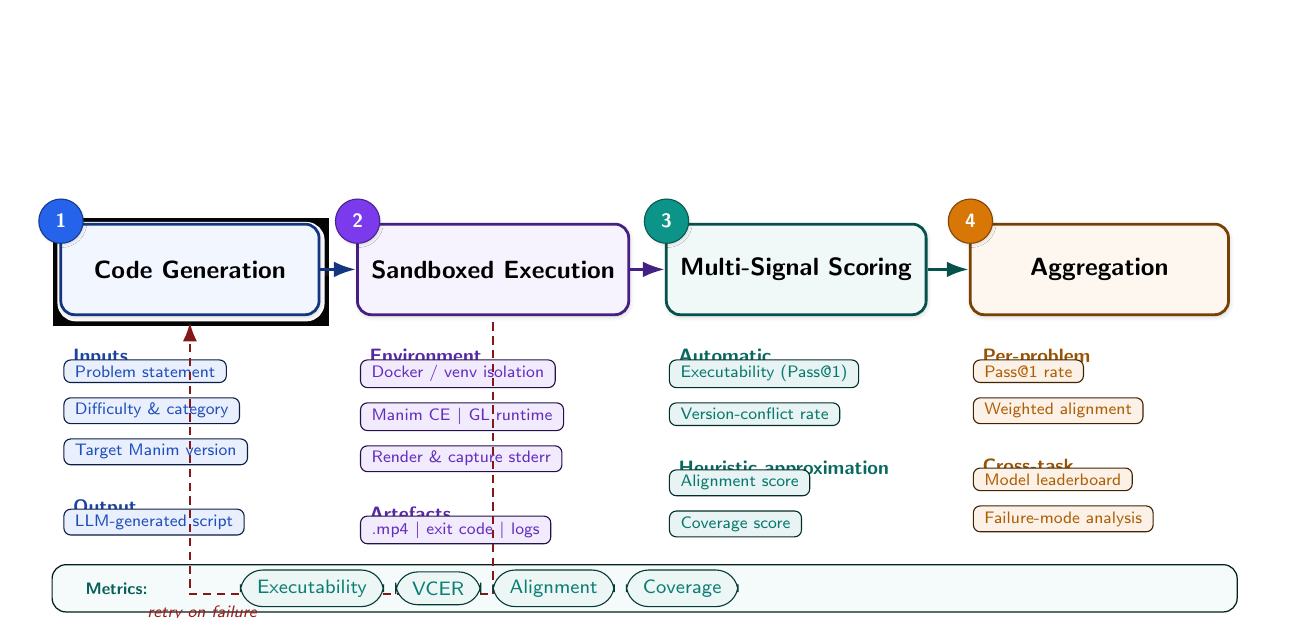
\begin{tikzpicture}[
        font=\sffamily\small,
        >=Latex,
    ]
        % ── Color palette ─────────────────────────────────────
        \definecolor{wfblue}{HTML}{2563EB}
        \definecolor{wfviolet}{HTML}{7C3AED}
        \definecolor{wfteal}{HTML}{0D9488}
        \definecolor{wforange}{HTML}{D97706}
        \definecolor{wfred}{HTML}{DC2626}
        \definecolor{panelbg}{HTML}{F8FAFC}
        \definecolor{panelborder}{HTML}{CBD5E1}
        \definecolor{trackgray}{HTML}{E2E8F0}

        % ── Shared styles ─────────────────────────────────────
        \tikzset{
            stage/.style 2 args={
                rectangle,
                rounded corners=5pt,
                draw=#1!55!black,
                line width=1pt,
                fill=#1!6,
                minimum width=3.28cm,
                minimum height=1.15cm,
                align=center,
                inner sep=5pt,
                blur shadow={shadow blur steps=6,
                             shadow xshift=0.4pt,
                             shadow yshift=-0.8pt,
                             shadow blur radius=1.6pt,
                             shadow opacity=18},
            },
            badge/.style 2 args={
                circle,
                draw=#1!60!black,
                fill=#1,
                text=white,
                inner sep=0pt,
                minimum size=16pt,
                font=\sffamily\scriptsize\bfseries,
                blur shadow={shadow blur steps=4,
                             shadow xshift=0.3pt,
                             shadow yshift=-0.5pt,
                             shadow blur radius=1pt,
                             shadow opacity=14},
            },
            bullet/.style 2 args={
                rectangle,
                rounded corners=2.5pt,
                draw=#1!30!black,
                fill=#1!10,
                inner xsep=4pt,
                inner ysep=2pt,
                font=\sffamily\fontsize{6.5}{8}\selectfont,
                text=#1!80!black,
            },
            metricpill/.style={
                rectangle,
                rounded corners=8pt,
                draw=wfteal!40!black,
                fill=wfteal!8,
                inner xsep=6pt,
                inner ysep=3.5pt,
                font=\sffamily\fontsize{6.8}{8.5}\selectfont,
                text=wfteal!85!black,
            },
            connector/.style={
                -{Latex[length=2.8mm, width=2mm]},
                line width=1.2pt,
                draw=#1!55!black,
            },
            feedbackarrow/.style={
                -{Latex[length=2.4mm, width=1.8mm]},
                line width=0.9pt,
                draw=wfred!60!black,
                densely dashed,
            },
            headerlabel/.style={
                font=\sffamily\fontsize{7.5}{9}\selectfont\bfseries,
                text=#1!70!black,
            },
        }

        % ── Coordinates ───────────────────────────────────────
        \coordinate (origin) at (0,0);
        \def\xsep{3.85}

        % ── Background panel ──────────────────────────────────
        \begin{scope}[on background layer]
            \fill[panelbg, rounded corners=8pt, draw=panelborder, line width=0.6pt]
                (-2.05, -4.55) rectangle ($(origin)+(\xsep*3+2.05, 2.55)$);
            % Title bar
            \fill[white, rounded corners=8pt]
                (-1.85, 1.95) rectangle ($(origin)+(\xsep*3+1.85, 2.38)$);
            \node[font=\sffamily\fontsize{7.8}{9}\selectfont\bfseries, text=black!60]
                at ($(origin)+(0.5*\xsep*3, 2.16)$)
                {\textsc{ManiBench} Evaluation Pipeline};
            % Horizontal track line
            \draw[trackgray, line width=2.8pt, line cap=round]
                (0, 0) -- +(\xsep*3, 0);
        \end{scope}

        % ══════════════════════════════════════════════════════
        % Stage 1 — Code Generation
        % ══════════════════════════════════════════════════════
        \node[stage={wfblue}{}] (gen) at (0,0)
            {\textbf{Code Generation}};

        \node[badge={wfblue}{}] at ($(gen.north west)+(0.02,0.02)$) {1};

        % Sub-items
        \node[headerlabel=wfblue, anchor=north west]
            at ($(gen.south west)+(0.05,-0.30)$) {Inputs};
        \node[bullet={wfblue}{}, anchor=north west] (g1)
            at ($(gen.south west)+(0.05,-0.55)$)
            {Problem statement};
        \node[bullet={wfblue}{}, anchor=north west] (g2)
            at ($(g1.south west)+(0,-0.18)$)
            {Difficulty \& category};
        \node[bullet={wfblue}{}, anchor=north west] (g3)
            at ($(g2.south west)+(0,-0.18)$)
            {Target Manim version};

        \node[headerlabel=wfblue, anchor=north west]
            at ($(g3.south west)+(0,-0.32)$) {Output};
        \node[bullet={wfblue}{}, anchor=north west] (g4)
            at ($(g3.south west)+(0,-0.55)$)
            {LLM-generated script};

        % ══════════════════════════════════════════════════════
        % Stage 2 — Sandboxed Execution
        % ══════════════════════════════════════════════════════
        \node[stage={wfviolet}{}] (exec) at (\xsep,0)
            {\textbf{Sandboxed Execution}};

        \node[badge={wfviolet}{}] at ($(exec.north west)+(0.02,0.02)$) {2};

        \node[headerlabel=wfviolet, anchor=north west]
            at ($(exec.south west)+(0.05,-0.30)$) {Environment};
        \node[bullet={wfviolet}{}, anchor=north west] (e1)
            at ($(exec.south west)+(0.05,-0.55)$)
            {Docker / venv isolation};
        \node[bullet={wfviolet}{}, anchor=north west] (e2)
            at ($(e1.south west)+(0,-0.18)$)
            {Manim CE \textbar{} GL runtime};
        \node[bullet={wfviolet}{}, anchor=north west] (e3)
            at ($(e2.south west)+(0,-0.18)$)
            {Render \& capture stderr};

        \node[headerlabel=wfviolet, anchor=north west]
            at ($(e3.south west)+(0,-0.32)$) {Artefacts};
        \node[bullet={wfviolet}{}, anchor=north west] (e4)
            at ($(e3.south west)+(0,-0.55)$)
            {.mp4 \textbar{} exit code \textbar{} logs};

        % ══════════════════════════════════════════════════════
        % Stage 3 — Multi-Signal Scoring
        % ══════════════════════════════════════════════════════
        \node[stage={wfteal}{}] (metric) at (2*\xsep,0)
            {\textbf{Multi-Signal Scoring}};

        \node[badge={wfteal}{}] at ($(metric.north west)+(0.02,0.02)$) {3};

        \node[headerlabel=wfteal, anchor=north west]
            at ($(metric.south west)+(0.05,-0.30)$) {Automatic};
        \node[bullet={wfteal}{}, anchor=north west] (s1)
            at ($(metric.south west)+(0.05,-0.55)$)
            {Executability (Pass@1)};
        \node[bullet={wfteal}{}, anchor=north west] (s2)
            at ($(s1.south west)+(0,-0.18)$)
            {Version-conflict rate};

        \node[headerlabel=wfteal, anchor=north west]
            at ($(s2.south west)+(0,-0.32)$) {Heuristic approximation};
        \node[bullet={wfteal}{}, anchor=north west] (s3)
            at ($(s2.south west)+(0,-0.55)$)
            {Alignment score};
        \node[bullet={wfteal}{}, anchor=north west] (s4)
            at ($(s3.south west)+(0,-0.18)$)
            {Coverage score};

        % ══════════════════════════════════════════════════════
        % Stage 4 — Aggregation & Reporting
        % ══════════════════════════════════════════════════════
        \node[stage={wforange}{}] (agg) at (3*\xsep,0)
            {\textbf{Aggregation}};

        \node[badge={wforange}{}] at ($(agg.north west)+(0.02,0.02)$) {4};

        \node[headerlabel=wforange, anchor=north west]
            at ($(agg.south west)+(0.05,-0.30)$) {Per-problem};
        \node[bullet={wforange}{}, anchor=north west] (a1)
            at ($(agg.south west)+(0.05,-0.55)$)
            {Pass@1 rate};
        \node[bullet={wforange}{}, anchor=north west] (a2)
            at ($(a1.south west)+(0,-0.18)$)
            {Weighted alignment};

        \node[headerlabel=wforange, anchor=north west]
            at ($(a2.south west)+(0,-0.32)$) {Cross-task};
        \node[bullet={wforange}{}, anchor=north west] (a3)
            at ($(a2.south west)+(0,-0.55)$)
            {Model leaderboard};
        \node[bullet={wforange}{}, anchor=north west] (a4)
            at ($(a3.south west)+(0,-0.18)$)
            {Failure-mode analysis};

        % ══════════════════════════════════════════════════════
        % Connectors between stages (gradient-coloured)
        % ══════════════════════════════════════════════════════
        \draw[connector=wfblue]
            (gen.east) -- (exec.west);
        \draw[connector=wfviolet]
            (exec.east) -- (metric.west);
        \draw[connector=wfteal]
            (metric.east) -- (agg.west);

        % ── Feedback loop (retry on failure) ──────────────────
        \draw[feedbackarrow]
            ($(exec.south)+(0,-0.08)$)
            -- ++(0,-3.45)
            -| ($(gen.south)-(0,0.08)$)
            node[pos=0.48, below=0.5pt, font=\sffamily\fontsize{6}{7.5}\selectfont\itshape,
                 text=wfred!70!black] {retry on failure};

        % ══════════════════════════════════════════════════════
        % Metric pills — bottom banner
        % ══════════════════════════════════════════════════════
        \begin{scope}[on background layer]
            \fill[wfteal!4, rounded corners=5pt, draw=wfteal!20!black, line width=0.45pt]
                ($(origin)+(-1.75,-3.75)$)
                rectangle ($(origin)+(\xsep*3+1.75,-4.35)$);
        \end{scope}

        \node[font=\sffamily\fontsize{6.5}{8}\selectfont\bfseries, text=wfteal!65!black,
              anchor=west]
            at ($(origin)+(-1.45,-4.05)$) {Metrics:};

        \node[metricpill] (mp1) at ($(origin)+(1.55,-4.05)$)
            {Executability};
        \node[metricpill, right=4pt of mp1] (mp2)
            {VCER};
        \node[metricpill, right=4pt of mp2] (mp3)
            {Alignment};
        \node[metricpill, right=4pt of mp3] (mp4)
            {Coverage};

    \end{tikzpicture}
    \caption{The \textsc{ManiBench} evaluation pipeline.
    Each benchmark problem flows through four stages:
    \emph{(1)}~an LLM generates Manim code from a structured prompt;
    \emph{(2)}~the script executes inside a sandboxed, version-pinned environment;
    \emph{(3)}~automatic checks (executability, version-conflict rate) and heuristic
    approximations (alignment, coverage) produce multi-signal scores; and
    \emph{(4)}~results are aggregated into per-problem and cross-task summaries.
    A dashed feedback loop indicates re-prompting on execution failure.}
    \label{fig:workflow}
\end{figure}

\subsection{Evaluation Scope}
\label{sec:eval-scope}

All four metrics in the current evaluation are computed \emph{fully automatically}.
Executability and VCER are determined via AST parsing, subprocess rendering, and regex-based static analysis.
Alignment and Coverage are approximated through keyword-bank and pattern-matching heuristics that detect the \emph{presence} of required visual events and pedagogical elements in the generated source code.
Because these heuristics operate on code tokens rather than rendered output, they serve as \textbf{conservative lower-bound estimates}: a keyword match confirms that a concept is referenced but cannot verify that it is correctly animated.

\noindent\textbf{Planned Human Evaluation.}
A structured human review protocol is designed for future work:
\begin{enumerate}[nosep]
    \item Watch the rendered animation.
    \item Check off each required visual event as present or absent.
    \item Assess timing synchronization and pedagogical clarity.
    \item Provide Alignment and Coverage scores ($0.0$--$1.0$).
\end{enumerate}
This protocol will employ two independent reviewers per output, with a third reviewer resolving disagreements exceeding~$0.15$, and inter-rater agreement reported via Krippendorff's~$\alpha$.
The current study reports only automated heuristic scores; no human evaluation has been conducted.


\subsection{Automated Evaluation Framework}
\label{sec:auto-eval}

We implement a fully automated evaluation pipeline for reproducible, large-scale metric computation.
The framework orchestrates code generation across multiple LLMs via the OpenRouter API, executes generated code in sandboxed environments, and computes all four metrics programmatically.

\subsubsection{Multi-Model Evaluation}

The pipeline supports evaluation across two API providers: OpenRouter (for commercial and large-scale models) and Inference.net (for self-hosted open-weight models).
Table~\ref{tab:models} lists the full model roster.

\begin{table}[ht]
    \centering
    \caption{Model roster for automated evaluation.
    Models are accessed via OpenRouter or Inference.net.
    The ``Eval.'' column indicates which evaluation runs were completed:
    Z = zero-shot only; A = all five prompting strategies.}
    \label{tab:models}
    \small
    \begin{tabular}{@{}lllc@{}}
        \toprule
        \textbf{Model} & \textbf{Provider} & \textbf{API} & \textbf{Eval.} \\
        \midrule
        \multicolumn{4}{@{}l}{\emph{OpenRouter models}} \\
        Kimi-K2.5           & Moonshot AI & OpenRouter & Z \\
        Qwen3.5-Plus        & Alibaba     & OpenRouter & Z \\
        Qwen3-235B-A22B     & Alibaba     & OpenRouter & Z \\
        Llama-3.1-8B        & Meta        & OpenRouter & Z \\
        Qwen-2.5-Coder-32B  & Alibaba     & OpenRouter & Z \\
        \midrule
        \multicolumn{4}{@{}l}{\emph{Inference.net models}} \\
        Gemma-3-27B         & Google      & Inference.net & A \\
        \bottomrule
    \end{tabular}
\end{table}

All models are evaluated with temperature~$0.0$ for reproducibility, with a maximum of 8{,}192~generated tokens per request.
OpenRouter models are evaluated with 1~trial per (model, problem) pair under zero-shot prompting.
Gemma-3-27B is evaluated with 3~trials across all five prompting strategies (Section~\ref{sec:prompt-strategies}), yielding $3 \times 12 \times 5 = 180$~total runs for the ablation study.

\subsubsection{Automated Metric Computation}

Each generated code sample passes through a four-stage analysis pipeline:

\begin{enumerate}[nosep]
    \item \textbf{Syntax Validation:} Python AST parsing (\texttt{ast.parse}) to verify syntactic correctness.
    \item \textbf{Structural Checks:} detection of at least one \texttt{Scene} subclass and valid \texttt{from manim import *} imports; flagging of ManimGL-specific imports.
    \item \textbf{Sandboxed Execution:} the code is written to a temporary file and rendered via \texttt{subprocess} with a configurable timeout (default: 60\,s).
    Exit codes, \texttt{stderr}, and error types (\texttt{ImportError}, \texttt{AttributeError}, etc.) are captured.
    \item \textbf{Static Analysis:} over 40~regex patterns (derived from the 145~documented GL$\to$CE incompatibilities in Section~\ref{sec:refcode}) scan for version conflicts; keyword-bank--based heuristics detect the presence of required visual events and pedagogical elements.
\end{enumerate}

\noindent All four metrics are computed fully automatically.
Executability and VCER use AST parsing, subprocess execution, and regex-based static analysis.
Alignment and Coverage are approximated heuristically via keyword and pattern matching, serving as conservative lower-bound estimates (see Section~\ref{sec:eval-scope}).


\subsection{Prompt Engineering Strategies}
\label{sec:prompt-strategies}

Following the ManiBench Prompt Engineering Guide, we implement five prompting strategies of increasing sophistication, each evaluated in full on Gemma-3-27B with 3~trials per problem:

\begin{enumerate}[nosep]
    \item \textbf{Zero-Shot Direct.}
    The problem statement is provided verbatim with a system prompt specifying Manim~CE as the target.
    Serves as the baseline across all models; Kimi-K2.5 achieves $66.7\%$ executability under this strategy.

    \item \textbf{Few-Shot Examples.}
    One or two working Manim~CE code examples precede the target problem.
    Examples are kept short (20--30~lines) and domain-relevant.
    In our ablation (Section~\ref{sec:ablation}), few-shot is the only strategy to improve executability for Gemma-3-27B ($+11.1$~pp) and yields a modest coverage gain ($+2.8$~pp).

    \item \textbf{Chain-of-Thought (CoT).}
    The model is instructed to first analyze visual components, event ordering, transformations, timing, and required labels before writing code.
    Empirically, CoT introduces a small version-conflict rate ($2.8\%$) on Gemma-3-27B and slightly degrades coverage, suggesting the reasoning trace can lead to deprecated API references.

    \item \textbf{Constraint-Based.}
    Explicit timing, ordering, and criticality constraints are injected (e.g., ``gradient arrow must appear \emph{before} dot moves'').
    Aimed at Level~3--4 problems; in practice, yields marginal changes in coverage and does not improve executability for Gemma-3-27B.

    \item \textbf{Version-Conflict-Aware.}
    The system prompt enumerates forbidden ManimGL constructs (derived from Section~\ref{sec:refcode}), and problem-specific incompatibilities from the dataset's \texttt{version\_conflict\_notes} field are appended.
    Eliminates version-conflict errors entirely for Gemma-3-27B ($\text{VCER} = 0.0\%$) and achieves perfect heuristic alignment ($1.0$).
\end{enumerate}


%% ═══════════════════════════════════════════════════════════════
\section{Results}
\label{sec:results}

\subsection{Experimental Setup}
\label{sec:setup}

\noindent\textbf{Models.}
We evaluate six models across two API providers (Table~\ref{tab:models}).
Five models are accessed via OpenRouter under zero-shot prompting with a single trial per (model, problem) pair, yielding $5 \times 12 = 60$~samples.
Gemma-3-27B is evaluated via Inference.net across all five prompting strategies with 3~trials each, yielding $180$~additional samples.
The total evaluation corpus comprises $240$~generated code samples.

\noindent\textbf{Environment.}
All code targets Manim~CE, executed in a sandboxed environment with a 60-second rendering timeout.
Metrics are computed using the automated pipeline described in Section~\ref{sec:auto-eval}.
Alignment and Coverage scores reported here are heuristic lower-bound estimates based on keyword and pattern matching; no human evaluation has been conducted in this study.


\subsection{Cross-Model Comparison (Zero-Shot)}
\label{sec:cross-model}

Table~\ref{tab:cross-model} reports aggregate results for all six models under zero-shot prompting.

\begin{table}[ht]
    \centering
    \caption{Cross-model comparison under zero-shot prompting.
    Executability (Exec.) is the fraction of outputs that render without error.
    VCER is the version-conflict error rate.
    Alignment (Align.) and Coverage (Cov.) are heuristic estimates.
    Best value in each column is \textbf{bolded}.}
    \label{tab:cross-model}
    \small
    \begin{tabular}{@{}llcccc@{}}
        \toprule
        \textbf{Model} & \textbf{API} & \textbf{Exec.~$\uparrow$} & \textbf{VCER~$\downarrow$} & \textbf{Align.~$\uparrow$} & \textbf{Cov.~$\uparrow$} \\
        \midrule
        Kimi-K2.5        & OpenRouter    & \textbf{0.667} & 0.083 & 0.917 & \textbf{0.265} \\
        Qwen3.5-Plus     & OpenRouter    & 0.333          & 0.085 & 0.917 & 0.226 \\
        Qwen3-235B-A22B  & OpenRouter    & 0.250          & \textbf{0.000} & \textbf{0.993} & 0.251 \\
        Llama-3.1-8B     & OpenRouter    & 0.083          & 0.024 & \textbf{1.000} & 0.132 \\
        Qwen-2.5-Coder   & OpenRouter    & 0.000          & \textbf{0.000} & 0.471 & 0.014 \\
        Gemma-3-27B      & Inference.net & 0.000          & \textbf{0.000} & 0.993 & 0.172 \\
        \bottomrule
    \end{tabular}
\end{table}

\noindent\textbf{Key Findings.}
Kimi-K2.5 achieves the highest executability ($66.7\%$), successfully rendering 8~of~12 problems.
Qwen3-235B-A22B and Gemma-3-27B produce zero version-conflict errors but struggle with executability ($25.0\%$ and $0.0\%$, respectively).
Qwen-2.5-Coder-32B fails to render any problem, with alignment scores averaging only $0.47$, indicating both structural and semantic deficiencies in its Manim code.
Notably, Llama-3.1-8B achieves a perfect alignment score of~$1.0$ (heuristic) despite only $8.3\%$ executability, suggesting its outputs contain the expected visual-event keywords even when the code does not execute.


\subsection{Per-Problem Analysis (Zero-Shot)}
\label{sec:per-problem}

Table~\ref{tab:per-problem} breaks down results by benchmark problem, averaged across all six models.

\begin{table}[ht]
    \centering
    \caption{Per-problem results averaged across all six models (zero-shot prompting).
    Diff.\ = difficulty level (1--5).}
    \label{tab:per-problem}
    \small
    \begin{tabular}{@{}llccccc@{}}
        \toprule
        \textbf{ID} & \textbf{Problem} & \textbf{Diff.} & \textbf{Exec.} & \textbf{VCER} & \textbf{Align.} & \textbf{Cov.} \\
        \midrule
        MB-001 & Colliding Blocks  & 4 & 0.17 & 0.012 & 0.89 & 0.25 \\
        MB-002 & Gradient Descent   & 3 & 0.00 & 0.003 & 0.86 & 0.15 \\
        MB-003 & Convolution        & 3 & 0.50 & 0.000 & 0.94 & 0.16 \\
        MB-004 & Eigenvectors       & 4 & 0.17 & 0.167 & 0.60 & 0.10 \\
        MB-005 & Determinant        & 2 & 0.17 & 0.000 & 0.88 & 0.16 \\
        MB-006 & CLT                & 3 & 0.33 & 0.000 & 0.90 & 0.18 \\
        MB-007 & Medical Test       & 2 & 0.50 & 0.000 & 0.92 & 0.19 \\
        MB-008 & Chain Rule         & 3 & 0.33 & 0.167 & 0.68 & 0.14 \\
        MB-009 & Integration        & 3 & 0.17 & 0.000 & 0.84 & 0.25 \\
        MB-010 & Taylor Series      & 4 & 0.17 & 0.000 & 0.92 & 0.24 \\
        MB-011 & Hairy Ball         & 5 & 0.00 & 0.000 & 0.88 & 0.17 \\
        MB-012 & Windmill           & 4 & 0.17 & 0.036 & 1.00 & 0.16 \\
        \bottomrule
    \end{tabular}
\end{table}


\subsection{Prompting Strategy Ablation (Gemma-3-27B)}
\label{sec:ablation}

Gemma-3-27B is the only model evaluated across all five prompting strategies (3~trials each), enabling a controlled ablation study.
Table~\ref{tab:ablation} reports the results.

\begin{table}[ht]
    \centering
    \caption{Prompting strategy ablation on Gemma-3-27B (3~trials per problem, 12~problems).
    Few-shot prompting yields the only non-zero executability.
    $\Delta$~columns report the change relative to zero-shot.}
    \label{tab:ablation}
    \small
    \begin{tabular}{@{}lcccccc@{}}
        \toprule
        \textbf{Strategy} & \textbf{Exec.} & \textbf{$\Delta$Exec.} & \textbf{VCER} & \textbf{Align.} & \textbf{Cov.} & \textbf{$\Delta$Cov.} \\
        \midrule
        Zero-Shot        & 0.000 & ---            & 0.000 & 0.993 & 0.172 & ---            \\
        Few-Shot         & \textbf{0.111} & $+11.1$ pp & 0.000 & \textbf{1.000} & \textbf{0.200} & $+2.8$ pp  \\
        Chain-of-Thought & 0.000 & $+0.0$ pp  & 0.028 & 0.972 & 0.159 & $-1.3$ pp  \\
        Constraint       & 0.000 & $+0.0$ pp  & 0.000 & 0.995 & 0.171 & $-0.1$ pp  \\
        Version-Aware    & 0.000 & $+0.0$ pp  & \textbf{0.000} & \textbf{1.000} & 0.175 & $+0.3$ pp  \\
        \bottomrule
    \end{tabular}
\end{table}

\noindent\textbf{Ablation Findings.}
\begin{enumerate}[nosep]
    \item \textbf{Few-shot is the only strategy that improves executability} for Gemma-3-27B, achieving $11.1\%$ Pass@1 (4~of~36 runs render successfully), concentrated on MB-006 (CLT), MB-007 (Medical Test), and MB-008 (Chain Rule).
    \item \textbf{Chain-of-thought introduces version conflicts} ($\text{VCER} = 2.8\%$) and slightly degrades alignment ($0.972$ vs.\ $0.993$).
    The reasoning trace appears to cause the model to reference deprecated constructs.
    \item \textbf{Version-aware prompting eliminates version conflicts} and achieves perfect heuristic alignment ($1.0$), confirming that explicit forbidden-construct lists are effective.
    \item \textbf{Coverage remains uniformly low} ($0.16$--$0.20$) across all strategies, indicating that prompting alone cannot substantially increase the density of pedagogical elements (mathematical annotations, numeric evidence, structural clarity).
\end{enumerate}


\subsection{Detailed Per-Model Per-Problem Grid}
\label{sec:grid}

Table~\ref{tab:grid} presents the full executability and coverage grid for the three highest-performing OpenRouter models and Gemma-3-27B.

\begin{table}[ht]
    \centering
    \caption{Per-model per-problem executability and coverage scores (zero-shot).
    Exec.\ values are binary (1~or~0) for single-trial OpenRouter runs; averaged over 3~trials for Gemma-3-27B.
    $\bullet$ = executable, $\circ$ = not executable.}
    \label{tab:grid}
    \small
    \setlength{\tabcolsep}{4pt}
    \begin{tabular}{@{}l *{4}{cc} @{}}
        \toprule
        & \multicolumn{2}{c}{\textbf{Kimi-K2.5}} & \multicolumn{2}{c}{\textbf{Qwen3.5+}} & \multicolumn{2}{c}{\textbf{Qwen3-235B}} & \multicolumn{2}{c}{\textbf{Gemma-3-27B}} \\
        \cmidrule(lr){2-3} \cmidrule(lr){4-5} \cmidrule(lr){6-7} \cmidrule(lr){8-9}
        \textbf{Problem} & Ex. & Cov. & Ex. & Cov. & Ex. & Cov. & Ex. & Cov. \\
        \midrule
        MB-001 & $\bullet$ & .42 & $\circ$ & .27 & $\circ$ & .34 & $\circ$ & .28 \\
        MB-002 & $\circ$   & .21 & $\circ$ & .17 & $\circ$ & .21 & $\circ$ & .14 \\
        MB-003 & $\bullet$ & .20 & $\bullet$ & .17 & $\bullet$ & .26 & $\circ$ & .17 \\
        MB-004 & $\bullet$ & .25 & $\circ$ & .00 & $\circ$ & .13 & $\circ$ & .16 \\
        MB-005 & $\bullet$ & .24 & $\circ$ & .22 & $\circ$ & .17 & $\circ$ & .12 \\
        MB-006 & $\bullet$ & .25 & $\bullet$ & .27 & $\circ$ & .25 & $\circ$ & .10 \\
        MB-007 & $\bullet$ & .32 & $\bullet$ & .23 & $\circ$ & .25 & $\circ$ & .13 \\
        MB-008 & $\circ$   & .00 & $\bullet$ & .33 & $\bullet$ & .26 & $\circ$ & .19 \\
        MB-009 & $\circ$   & .36 & $\circ$ & .38 & $\bullet$ & .39 & $\circ$ & .24 \\
        MB-010 & $\bullet$ & .33 & $\circ$ & .31 & $\circ$ & .27 & $\circ$ & .22 \\
        MB-011 & $\circ$   & .27 & $\circ$ & .21 & $\circ$ & .24 & $\circ$ & .18 \\
        MB-012 & $\bullet$ & .34 & $\circ$ & .15 & $\circ$ & .25 & $\circ$ & .14 \\
        \midrule
        \textbf{Mean} & \textbf{.67} & \textbf{.27} & .33 & .23 & .25 & .25 & .00 & .17 \\
        \bottomrule
    \end{tabular}
\end{table}


\subsection{Key Observations}
\label{sec:observations}

\begin{enumerate}[nosep]
    \item \textbf{Executability is the primary bottleneck.}
    Even the best-performing model (Kimi-K2.5) renders only $66.7\%$ of problems.
    The expert-level Hairy Ball theorem (MB-011, difficulty~5) was not rendered by any model.
    \item \textbf{Version conflicts are sparse but concentrated.}
    Two problems trigger version-conflict errors across models: MB-004 (Eigenvectors, $\text{VCER} = 16.7\%$) and MB-008 (Chain Rule, $\text{VCER} = 16.7\%$), both involving linear-algebra transformations that tempt models into using deprecated \texttt{ShowCreation} or ManimGL-specific \texttt{CONFIG} patterns.
    \item \textbf{Heuristic alignment saturates.}
    Most models achieve alignment scores above $0.90$ because keyword-based detection cannot distinguish whether visual events are \emph{correctly implemented} versus merely \emph{mentioned in comments or string literals}.
    This underscores the need for future human review or vision-based evaluation to produce more discriminative alignment scores.
    \item \textbf{Coverage is uniformly low.}
    Average coverage across all models is $0.18$, indicating that LLM-generated Manim code lacks pedagogical richness---mathematical annotations, numeric evidence trackers, and structural clarity elements are rarely produced.
    \item \textbf{Model scale does not guarantee Manim proficiency.}
    Qwen3-235B-A22B (235B~parameters) achieves lower executability ($25.0\%$) than Kimi-K2.5, suggesting that domain-specific training data availability matters more than raw scale for specialized code generation.
\end{enumerate}


%% ═══════════════════════════════════════════════════════════════
\section{Discussion}
\label{sec:discussion}

\subsection{Why ManiBench Matters}

Existing benchmarks (HumanEval, APPS) measure whether code produces correct \emph{output}.
\textsc{ManiBench} measures whether code produces correct \emph{understanding}.
This distinction is critical for educational tools, where a silent failure (wrong animation) is worse than a loud failure (runtime error).

\subsection{Limitations and Future Work}

\begin{enumerate}[nosep]
    \item \textbf{No Human Evaluation.}
    All metrics reported in this study are computed fully automatically.
    Alignment and Coverage rely on keyword-bank and regex heuristics that detect concept \emph{presence} but cannot verify \emph{correctness} of the rendered animation.
    A structured human review protocol has been designed (Section~\ref{sec:eval-scope}) but not yet conducted; incorporating human judgments is a high-priority next step.
    \item \textbf{Heuristic Alignment Saturation.}
    The keyword-based alignment metric saturates near~$1.0$ for most models (Section~\ref{sec:observations}), failing to distinguish correct implementations from code that merely contains relevant keywords.
    Future work should integrate frame-level video comparison or vision--language model grading to produce more discriminative alignment scores.
    \item \textbf{Limited Model Coverage.}
    Due to API availability constraints, only Gemma-3-27B was evaluated across all five prompting strategies.
    OpenRouter models were evaluated under zero-shot prompting with a single trial.
    Extending to full multi-trial, multi-strategy evaluation for frontier models (GPT-4o, Claude~Sonnet~4, Gemini~2.5~Pro) is a priority.
    \item \textbf{Pedagogical Validation.}
    We do not yet validate whether animations actually teach the concept.
    User studies with students could address this gap.
    \item \textbf{Manim API Coverage.}
    As Manim evolves, the benchmark should be versioned and updated accordingly.
    The 145~documented GL$\to$CE incompatibilities provide a starting point for automated version-conflict detection.
    \item \textbf{Scalability.}
    Moving from 12 to 150+ problems requires annotation infrastructure and community contribution.
    \item \textbf{Reference Code Utilization.}
    The ${\sim}53{,}000$~lines of analyzed reference code could enable fine-tuning studies or retrieval-augmented generation (RAG) experiments.
\end{enumerate}

\subsection{Broader Impact}

\textsc{ManiBench} can be used to:
\begin{itemize}[nosep]
    \item evaluate LLM educational-content generation across model families and scales,
    \item develop better prompting strategies for animation code (our ablation shows few-shot is most effective for executability),
    \item identify systematic failure modes (e.g., uniformly low pedagogical coverage, version-conflict concentration on transformation-heavy problems),
    \item drive research into improving Manim API adoption in LLMs,
    \item benchmark version-aware code generation using the 145~documented GL$\to$CE incompatibilities, and
    \item enable retrieval-augmented generation (RAG) experiments using the reference code analysis.
\end{itemize}


%% ═══════════════════════════════════════════════════════════════
\section{Conclusion}
\label{sec:conclusion}

We have introduced \textsc{ManiBench}, a specialized benchmark for evaluating Manim code generation.
By formalizing metrics for syntactic correctness, version compliance, visual-logic alignment, and pedagogical coverage, \textsc{ManiBench} moves beyond simple test-case evaluation to assess whether generated animations actually communicate mathematical concepts.

The 12-problem pilot dataset, backed by comprehensive reference code analysis of ${\sim}53{,}000$~lines of original 3Blue1Brown source code and 145~documented GL$\to$CE incompatibilities, reveals that even the best-performing model (Kimi-K2.5) renders only $66.7\%$ of problems, while coverage of pedagogical elements averages just~$0.18$.
Our prompting strategy ablation on Gemma-3-27B shows that few-shot examples are the only strategy to measurably improve executability ($+11.1$~pp), while version-aware prompting effectively eliminates version-conflict errors.
The accompanying automated evaluation framework---supporting models across OpenRouter and Inference.net with five prompting strategies---enables reproducible assessment.
With planned expansion to 150--200 problems and integration of vision-based alignment scoring, \textsc{ManiBench} will serve as a foundational resource for advancing LLM-driven educational content creation.

The dataset and evaluation toolkit are publicly available at \url{https://huggingface.co/datasets/nabin2004/ManiBench}.


%% ═══════════════════════════════════════════════════════════════
\section*{References}
\label{sec:references}

\begin{enumerate}[nosep, label={[\arabic*]}]
    \item M.~Chen, J.~Tworek, H.~Jun, et al., ``Evaluating Large Language Models Trained on Code,'' \emph{arXiv:2107.03374}, 2021. (HumanEval)
    \item J.~Austin, A.~Odena, M.~Nye, et al., ``Program Synthesis with Large Language Models,'' \emph{arXiv:2108.07732}, 2021. (MBPP)
    \item D.~Hendrycks, S.~Basart, S.~Kadavath, et al., ``Measuring Coding Challenge Competence with APPS,'' \emph{NeurIPS Datasets and Benchmarks}, 2021.
    \item G.~Sanderson, ``3Blue1Brown,'' \url{https://www.3blue1brown.com/}, 2015--present.
    \item Manim Community Developers, ``Manim---Mathematical Animation Framework (Community Edition),'' \url{https://www.manim.community/}, 2020--present.
    \item G.~Sanderson, ``Manim (3Blue1Brown fork),'' \url{https://github.com/3b1b/manim}, 2015--present.
    \item T.~Brown, B.~Mann, N.~Ryder, et al., ``Language Models are Few-Shot Learners,'' \emph{NeurIPS}, 2020.
    \item J.~Wei, X.~Wang, D.~Schuurmans, et al., ``Chain-of-Thought Prompting Elicits Reasoning in Large Language Models,'' \emph{NeurIPS}, 2022.
    \item OpenAI, ``GPT-4o Technical Report,'' 2024.
    \item Anthropic, ``Claude Sonnet~4 Model Card,'' 2025.
    \item Google DeepMind, ``Gemini 2.5 Pro Technical Report,'' 2025.
    \item DeepSeek, ``DeepSeek-R1: Incentivizing Reasoning Capability in LLMs via Reinforcement Learning,'' \emph{arXiv:2501.12948}, 2025.
\end{enumerate}


%% ═══════════════════════════════════════════════════════════════
\appendix
\section{Problem Annotation Template}
\label{app:template}

Each problem in \textsc{ManiBench} is annotated as a JSON object with the following structured metadata:

\begin{description}[nosep]
    \item[\texttt{id}:] unique identifier (e.g., \texttt{MB-001}).
    \item[\texttt{title}:] descriptive title.
    \item[\texttt{youtube\_video\_id}:] YouTube video identifier.
    \item[\texttt{category}:] list of task categories (e.g., \texttt{["drift-sensitive", "multi-scene"]}).
    \item[\texttt{difficulty\_level}:] integer 1--5.
    \item[\texttt{domain}:] list of mathematical domain(s).
    \item[\texttt{full\_prompt}:] full natural-language problem statement (used as the LLM input).
    \item[\texttt{raw\_code\_status}:] whether original 3B1B source code has been collected.
    \item[\texttt{raw\_code\_path}:] relative path to original ManimGL source files.
    \item[\texttt{reference\_code\_analysis}:] structured analysis of original code, including:
    \begin{description}[nosep]
        \item[\texttt{framework}:] source framework (e.g., \texttt{manim\_gl}).
        \item[\texttt{total\_lines}:] lines of original code.
        \item[\texttt{scene\_classes}:] list of scene classes with descriptions and key methods.
        \item[\texttt{visual\_techniques}:] catalog of rendering and animation patterns.
        \item[\texttt{manim\_api\_patterns}:] updaters, animation types, 3D constructs, custom classes.
    \end{description}
    \item[\texttt{required\_visual\_events}:] list of events, each with an identifier, description, weight, criticality flag, timing, and reference code location.
    \item[\texttt{coverage\_requirements}:] list of required pedagogical elements.
    \item[\texttt{version\_conflict\_notes}:] GL$\to$CE incompatibilities specific to the problem.
    \item[\texttt{success\_criteria}:] minimum thresholds for executability, alignment, coverage, and version-conflict error rate.
    \item[\texttt{common\_failure\_modes}:] known LLM failure patterns with severity tags.
\end{description}

\noindent The full dataset is available in JSON format at \url{https://huggingface.co/datasets/nabin2004/ManiBench}.

\end{document}
